\documentclass[output=paper]{LSP/langsci}  
\author{Chitsuko Fukushima\affiliation{University of Niigata Prefecture, Faculty of International Studies and Regional Development}} 
\title{Tracing real and apparent time language changes by comparing linguistic maps}
 
% }

%\maketitle

\abstract{
Geographical distributions on linguistic maps show what language changes have occurred in a surveyed area. In Japan, two national geolinguistic surveys have been conducted in the past: the Linguistic Atlas of Japan (\citealt{national_language_research_institute_linguistic_1966}, \textsc{LAJ}) and the Grammar Atlas of Japanese Dialects (\citealt{national_language_research_institute_grammar_1989}, \textsc{GAJ}). Recently, a third nation-wide geolinguistic survey, the Field-Research Project for Analyzing the Formation Process of Japanese Dialects (\textsc{FPJD}) was conducted to analyze the current geographical distributions of the phonological, lexical, and grammatical items. The informants  in the surveys were  elderly people.  The data from the surveys conducted in different periods was compared, and real-time language changes occurring over the generations were traced. The regional geolinguistic data of the younger generation was also used for comparison to examine apparent-time changes. Thus linguistic maps from different surveys have been redrawn using the same symbols for comparison and then superimposed. The results of the study show two patterns of language change for completed changes and changes in progress.
}
\rohead{\thechapter\hspace{.5em} Tracing real and apparent time language changes}
\maketitle 
\begin{document}
\section{Introduction}
Geographical distributions on linguistic maps indicate what language changes have occurred in a surveyed area. To examine \isi{real-time changes}, a survey is repeated after a period of time, and, to observe \isi{apparent-time changes}, different generations are surveyed. \citet{fukushima_revisiting_2013} reported results of a comparison between two geolinguistic\is{geolinguistics} surveys of Tokunoshima dialects of Japanese. The two surveys were conducted 30 years apart with a focus on \isi{real-time changes}. Although it is difficult to repeat a geolinguistic survey with the same scope, especially on a national level, a nation-wide geolinguistic survey, the Field-Research Project for Analyzing the Formation Process of Japanese Dialects (\textsc{FPJD}), was conducted in Japan. The aim of this \isi{real-time interval research} is to compare the dialectal distributions from different surveys and to examine the interpretation of \isi{linguistic maps} from the older surveys \citep{onishi_timespan_2014}. In this paper, data from the national surveys and the recent regional survey of the young generation is compared to trace real- and apparent-time language changes.

\section{Data and Methods}

Three nation-wide geolinguistic surveys targeted at the elderly have been conducted in Japan to examine linguistic variation and change: (i) the Linguistic Atlas of Japan (\textsc{LAJ}), which mainly focused on lexical items and was conducted around 1960; (ii) the Grammar Atlas of Japanese Dialects (\textsc{GAJ}), which was exclusively concerned with grammatical items and was conducted around 1980; and (iii) the \textsc{FPJD}, which has recently been completed and which focuses on phonological, lexical, and grammatical items. A recent regional survey targeted at the younger generation, which includes phonological, lexical, and grammatical items, is the Survey of College Students in Niigata (\textsc{CS}) (see \tabref{tab:1}).

\begin{table}
\resizebox{\textwidth}{!}{
\begin{tabular}{lllllll}
\lsptoprule
{\bfseries Title} & 
{\bfseries Type} & 
{\bfseries Informants} & 
\begin{minipage}[t]{0.12\textwidth}\bfseries Time of survey\end{minipage} & 
\begin{minipage}[t]{0.12\textwidth}\bfseries \# of all-Japan localities\end{minipage} & 
\begin{minipage}[t]{0.12\textwidth}\bfseries \# of localities in Niigata\end{minipage} & 
\begin{minipage}[t]{0.2\textwidth}\bfseries Mean birth year of informants\end{minipage}\\
\midrule
{\mdseries \textsc{LAJ}} & {\mdseries National} & {\mdseries elderly} & {\mdseries 1957--1965} & {\mdseries 2400} & {\mdseries 91} & {\mdseries 1887}\\
{\mdseries \textsc{GAJ}} & {\mdseries National} & {\mdseries elderly} & {\mdseries 1979--1982} & {\mdseries 807} & {\mdseries 29} & {\mdseries 1916}\\
{\mdseries \textsc{FPJD}} & {\mdseries National} & {\mdseries elderly} & {\mdseries 2010--2014} & {\mdseries 554} & {\mdseries 22} & {\mdseries 1937}\\
{\mdseries \textsc{CS}} & {\mdseries Regional} & {\mdseries youth} & {\mdseries 1994--2002} & {\mdseries {}-} & {\mdseries 103 max.} & {\mdseries 1980 approx.}\\
\lspbottomrule
\end{tabular}
}
\caption{A comparison of characteristics of four surveys}\label{tab:1}
\end{table}

The data from the national surveys \textsc{LAJ} and \textsc{GAJ} was compared with that from \textsc{FPJD} to trace real-time changes, while the \textsc{FPJD} data was compared with that from \textsc{CS} to examine \isi{apparent-time changes}.  The \textsc{CS} informants were 631 college students from various localities in Niigata prefecture. To construct the \textsc{CS} maps such as \figref{fig:8}, \figref{fig:11} and \figref{fig:14} below, symbols were plotted at the location of each student's town of origin.

\begin{figure}
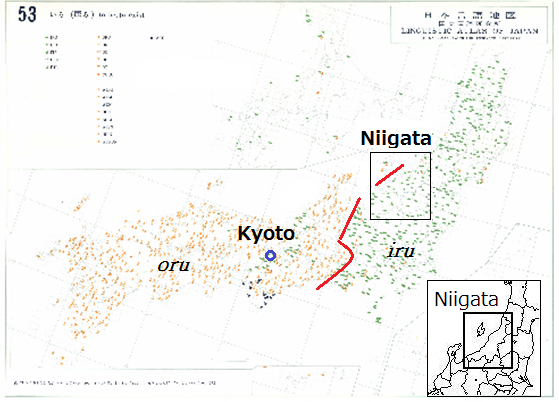
\includegraphics[width=1\textwidth]{illustrations/fuku2_fig1}
\caption{\textsc{LAJ} 53 \textit{iru} `to be or exist' and Niigata (Original map downloaded from \textsc{LAJ} Maps Download).}
\label{fig:1}
\end{figure}

The data examined here illustrate the dialectal variation in Niigata prefecture, where the border between Western and Eastern Japanese dialects is situated.\is{dialectal border} \figref{fig:1} shows a linguistic map for \textit{iru} `(a person) to be or exist' from \textsc{LAJ}.\footnote{\textsc{LAJ} Maps Download: \url{http://www.ninjal. ac.jp/publication/catalogue/laj\_map/}}.  The \isi{lexical variation} shown here is a contrastive East-West distribution pattern with a clear isogloss drawn just within Niigata prefecture.  The geographical distribution shows that the Western form has diffused from the central part of Japan where the old capital Kyoto is located.  A bundle of such isoglosses is found in Niigata prefecture, which shows the division between Western and Eastern dialects.

\citet{fukushima_superimposing_2007} compared geolinguistic survey results for Niigata dialects from two different surveys in order to examine linguistic variation and change.  Either \textsc{GAJ} or LAN --- the Linguistic Atlas of Niigata, a regional survey conducted by Katsuo Ohashi in 1980-1985 \citep{ohashi_linguistic_1998} --- was used as the data from the older generation, and \textsc{CS} was adopted as the data from the younger generation.  Two \isi{linguistic maps} were superimposed by using the SEAL 7.0J system developed by the author.\is{superimposing maps}  This paper compares geolinguistic survey results for Niigata dialects from three different surveys: \textsc{LAJ} or \textsc{GAJ}, \textsc{FPJD}, and \textsc{CS}.  The \textsc{GIS}\is{geographical information systems (GIS)} software SIS 7.1 was used to make comparable linguistic maps by adopting the same symbols and superimposing\is{superimposing maps} the distribution of relevant words from different surveys.  The results of the comparison are discussed in the following sections.

\section{Completed changes}\is{completed changes}

Figures 2--4 show changes that were completed in the past.  All three maps show East-West contrastive patterns with isoglosses in Niigata but do not show much difference over time.

\begin{figure}
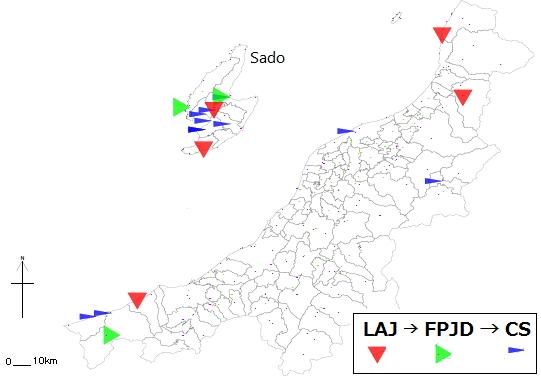
\includegraphics[width=.75\textwidth]{illustrations/fuku2_fig2a}
\caption{Diffusion of the Western form \textit{oru} for \textit{iru} `[a person] to be or exist'.}
\label{fig:2a}\is{diffusion}
\end{figure}

\begin{figure}
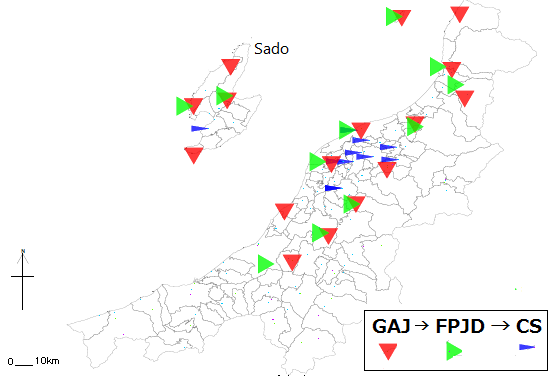
\includegraphics[width=.75\textwidth]{illustrations/fuku2_fig2b}
\caption{Diffusion of the Western form \textit{k\^{o}
%ː
ta} for \textit{katta} `bought [past tense]'.}
\label{fig:2b}\is{diffusion}
\end{figure}

\begin{figure}
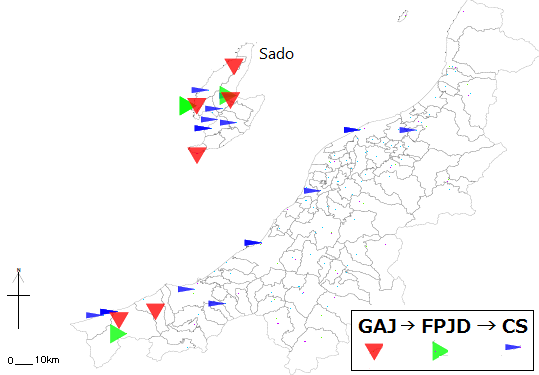
\includegraphics[width=.75\textwidth]{illustrations/fuku2_fig2c}
\caption{Diffusion of the Western forms \textit{sen}, \textit{sin} for \textit{sinai} `do not perform or act [a negative form]'.}
\label{fig:2c}\is{diffusion}
\end{figure}

%%%
%%% watch the IPA length signs in koːta, etc.
%%%
Each map shows the distribution of Western form(s) in \textsc{LAJ}/\textsc{GAJ} (red symbols), \textsc{FPJD} (green symbols), and \textsc{CS} (blue symbols).  \figref{fig:2a} maps the \isi{lexical variation} of \textit{iru} `(of a person) to be or exist'.  In \textsc{LAJ}, the Western form \textit{oru} is found on Sado Island, and in the westernmost and northernmost parts of mainland Niigata.  In \textsc{FPJD} and \textsc{CS}, the Western form is still found on Sado Island and in the westernmost part of mainland Niigata.  Thus the distributions do not vary much between \textsc{LAJ}, \textsc{FPJD} and \textsc{CS}.  \figref{fig:2b} maps the \isi{morphological variation} of \textit{katta} `bought [a past tense form of the verb `buy'].'  The Western form \textit{koːta} is found in \textsc{GAJ} on Sado Island and also in the central and northern parts of mainland Niigata (this area almost coincides with the Kambara Plains).  The distributions in \textsc{FPJD} are the same as those in \textsc{GAJ}, but those in \textsc{CS}, although located in the same area, are more restricted.  \figref{fig:2c} maps the \isi{morphological variation} of \textit{sinai} {\textquotedbl}do not perform [a negative form of the verb `perform'].{\textquotedbl} The Western forms \textit{sen} and \textit{sin} are distributed in \textsc{GAJ} on Sado Island and in the westernmost part of mainland Niigata. The distributions in \textsc{FPJD} are the same, but the distribution of the Western forms has expanded slightly  in mainland Niigata in \textsc{CS}.

These \isi{linguistic maps} show the contrastive distributions between Eastern dialect forms and Western dialect forms.  From the maps, we can conclude that Western dialect forms expanded to Sado Island and part of mainland Niigata in the past, but that they later lost their influence due to the spread of Eastern dialect forms, which happened to be the standard forms. The Eastern forms were maintained as the linguistic repertoire of the younger generation as a result of language \isi{standardization}. \figref{fig:2c} shows a slight expansion of the Western forms on the coast of mainland Niigata probably due to  competition from localized variants \textit{sine} and \textit{sin\^{e}ː} as well as a standard form \textit{sinai}.  

\begin{figure}
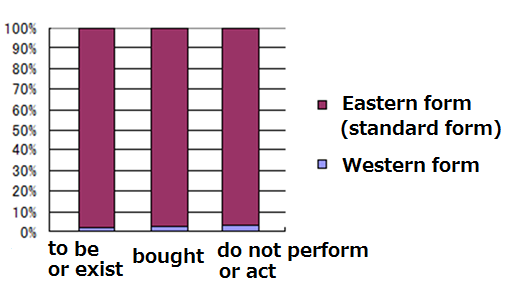
\includegraphics[width=.75\textwidth]{illustrations/fuku2_fig3}
\caption{Percentage of actual users of Western forms in the \textsc{CS} data.}
\label{fig:3}
\end{figure}

\figref{fig:3} confirms this interpretation, as users of Western dialect forms make up less than 5 percent of all \textsc{CS} informants.

\section{Changes in Progress}

\begin{figure}
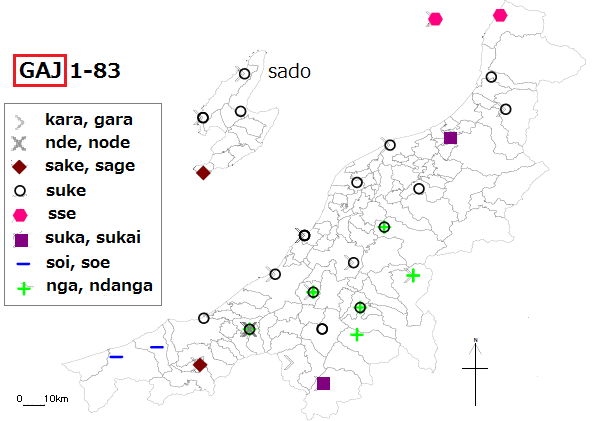
\includegraphics[width=0.75\textwidth]{illustrations/fuku2_fig4a}
\caption{\textit{kara} `because' from GAJ}
\label{fig:4a}
\end{figure}

\begin{figure}
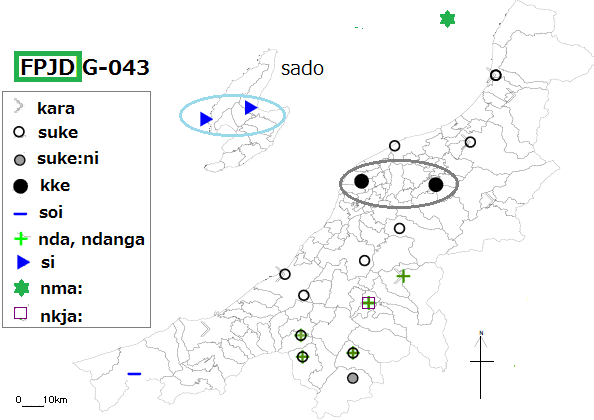
\includegraphics[width=0.75\textwidth]{illustrations/fuku2_fig4b}
\caption{\textit{kara} `because' from FPJD}
\label{fig:4b}
\end{figure}

\begin{figure}
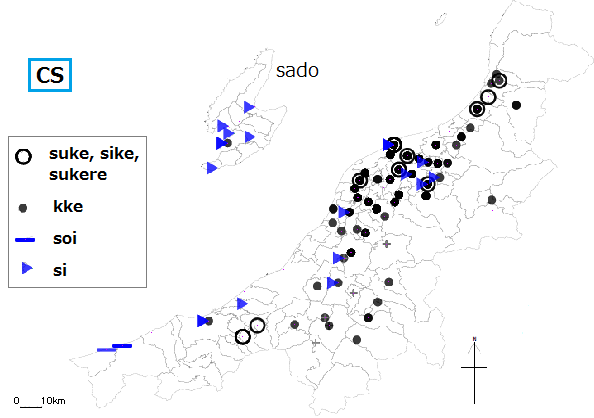
\includegraphics[width=0.75\textwidth]{illustrations/fuku2_fig4c}
\caption{\textit{kara} `because' from CS}
\label{fig:4c}
\end{figure}

The next group of maps shows \isi{changes in progress}. Here, the linguistic distributions in different surveys show conspicuous differences. 

\figref{fig:4a}, \figref{fig:4b}, and \figref{fig:4c} map the \isi{lexical variation} of \textit{kara} `because'  in \textsc{GAJ}, \textsc{FPJD}, and \textsc{CS} respectively.  Unlike the maps shown in the previous section, these maps show different distributions for the different surveys.  The traditional dialectal form \textit{suke} and its variants occupy most localities in \textsc{GAJ}.  The map for \textsc{FPJD} shows two new words, \textit{kke} and \textit{si}, both of which have increased their distribution as shown in the map for \textsc{CS}: the form \textit{kke} is a phonological derivation from \textit{suke}, and the form \textit{si} is a Western dialect form.  The \textsc{FPJD} map thus clearly indicates the beginning of \isi{lexical innovation}, which was expanded later.

\begin{figure}
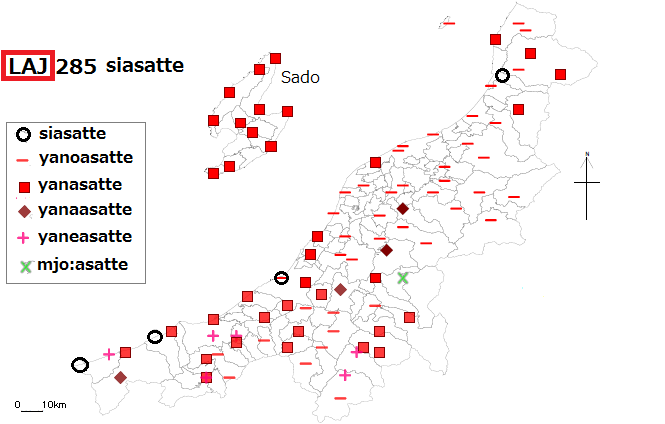
\includegraphics[width=.75\textwidth]{illustrations/fuku2_fig5a}
\caption{`two days after tomorrow' from LAJ}
\label{fig:5a}
\end{figure}

\begin{figure}
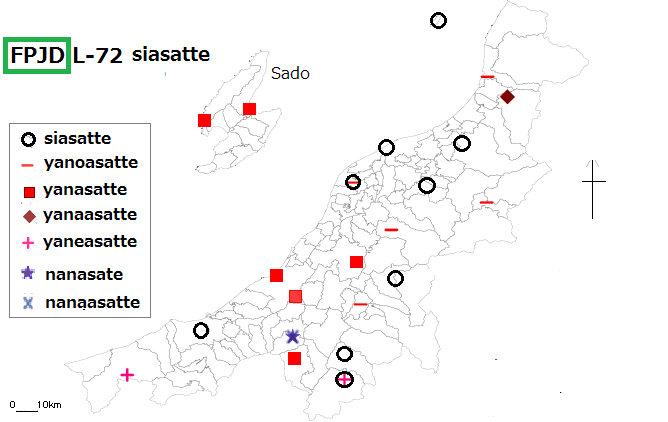
\includegraphics[width=.75\textwidth]{illustrations/fuku2_fig5b}
\caption{`two days after tomorrow' from FPJD}
\label{fig:5b}
\end{figure}

\begin{figure}
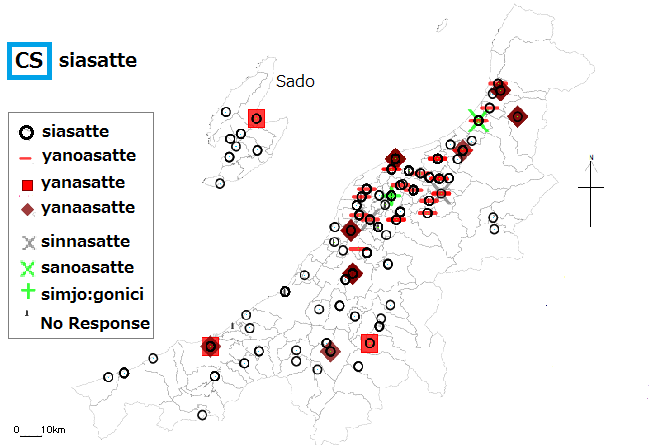
\includegraphics[width=.75\textwidth]{illustrations/fuku2_fig5c}
\caption{`two days after tomorrow' from CS}
\label{fig:5c}
\end{figure}

\begin{figure}
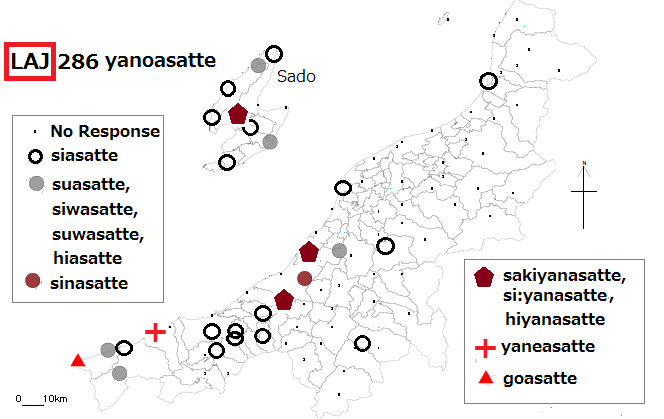
\includegraphics[width=.75\textwidth]{illustrations/fuku2_fig6a}
\caption{`three days after tomorrow' from LAJ}
\label{fig:6a}
\end{figure}

\begin{figure}
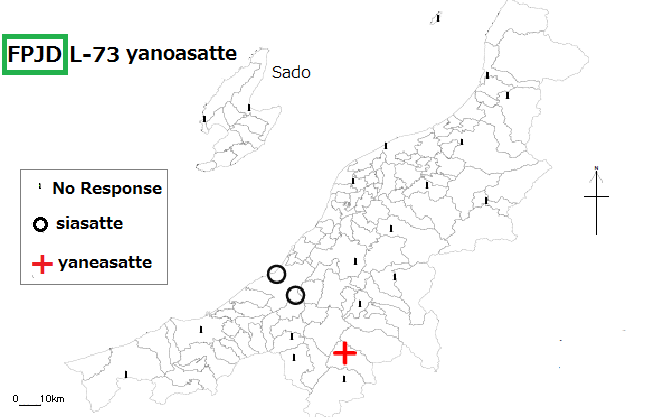
\includegraphics[width=.75\textwidth]{illustrations/fuku2_fig6b}
\caption{`three days after tomorrow' from  FPJD}
\label{fig:6b}
\end{figure}

\begin{figure}
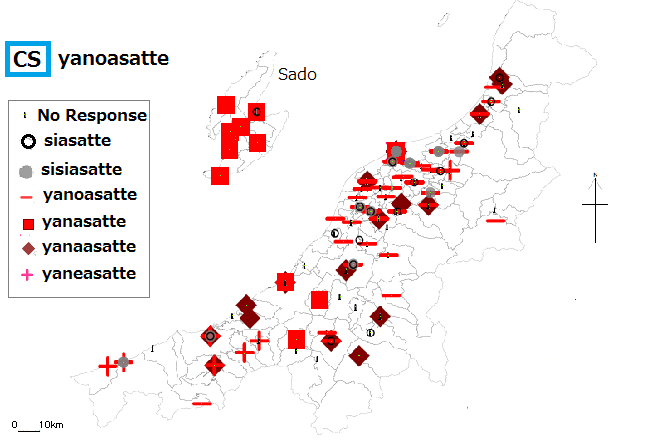
\includegraphics[width=.75\textwidth]{illustrations/fuku2_fig6c}
\caption{`three days after tomorrow' from CS}
\label{fig:6c}
\end{figure}

%\figref{fig:5a} through \figref{fig:6c} 
Figures 9--14 map the lexical changes in \textit{siasatte} `two days after tomorrow' and \textit{yanoasatte} `three days after tomorrow'.  For each lexical item, maps are shown from \textsc{LAJ}, \textsc{FPJD}, and \textsc{CS}. This pair of lexical items shows some interesting changes.  In \textsc{LAJ}, \figref{fig:5a} and \figref{fig:6a} show contrastive distributions between Eastern Niigata and Western Niigata (including Sado).  In Eastern Niigata, the traditional dialect had a localized form \textit{yanoasatte} which means `two days after tomorrow' but there was no equivalent word for `three days after tomorrow'; on the other hand, in Western Niigata, there were localized words, \textit{yanasatte, yanaasatte,} and \textit{yaneasatte} with the meaning of `two days after tomorrow', but \textit{siasatte} meant `three days after tomorrow', unlike in the \isi{standard system}. In \textsc{FPJD}, influenced by the system of standard Japanese, the standard word \textit{siasatte} was introduced with the meaning of `two days after tomorrow', but this resulted in a conflict with the \isi{localized system} especially in Western Niigata (see \figref{fig:5b} and \figref{fig:6b}).  In \textsc{CS}, some of the young generation adopted the \isi{standard system} but others used localized dialectal forms \textit{yanasatte, yanaasatte}, and \textit{yaneassatte} with the meaning of `three days after tomorrow' (see \figref{fig:5c} and \figref{fig:6c}). This has resulted in a new system, shown in \figref{fig:7}.

In both cases, the \textsc{FPJD} data shows the transitional stage of dialectal changes between the \textsc{LAJ}/\textsc{GAJ} data and the \textsc{CS} data. If the changes have occurred in the local area recently, they will be captured by the \textsc{FPJD} maps.

\begin{figure}
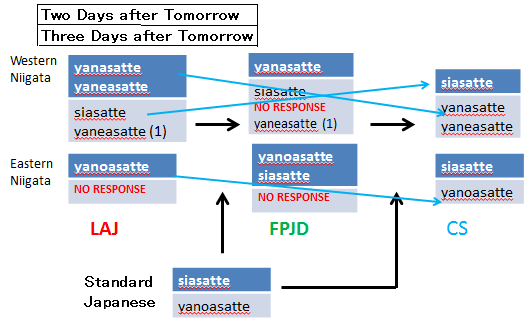
\includegraphics[width=0.6\textwidth]{illustrations/fuku2_fig7}
\caption{Changes of usage in {\textquotedbl}two days after tomorrow{\textquotedbl} and {\textquotedbl}three days after tomorrow{\textquotedbl}}
\label{fig:7}
\end{figure}

\section{Conclusion}

Regional language changes are traced back using data from three different geolinguistic surveys.  Two patterns of results are reported.  In the first case, the expansion of Western dialect forms is weakened due to language \isi{standardization}.  Changes were observed in the past but no additional advancement was reported in the \isi{linguistic maps}.  In the second case, local dialectal change is still on-going.  The recent nation-wide survey of elderly speakers has captured the transition in progress.  The results of the study show “a shift in focus from studying the spread of older linguistic features to studying the spread of innovative features” as observed by \citet[412]{gordon_changes_2000}.  Geographical Information Systems (\textsc{GIS})\is{geographical information systems (GIS)} are useful in statistical and quantitative analysis as stated by \citet{lee_spatial_1993}, while the \isi{georeferencing} function of \textsc{GIS} is used to compare and superimpose\is{superimposing maps} \isi{linguistic maps} from different surveys as reported in this paper.  The author has been involved in integrating or comparing the distribution patterns of linguistic features found in individual \isi{linguistic maps} with an objective to “describe” and “explain” or “adduce reasons for the distributions” \citep[216]{trudgill_linguistic_1974}.  Only a few common items from different surveys were compared in this paper, but the patterns reported should be seen as representative. When more data from the younger generation is available for comparison, this opens the way to quantitative analysis.

\section*{Acknowledgment}

This paper is part of the outcomes of the collaborative research project “Field-Research Project for Analyzing the Formation Process of Japanese Dialects”, carried out at the National Institute for Japanese Language and Linguistics, and was supported by Grant-in-Aid for Scientific Research (A) 23242024 and (C) 25370487.

\printbibliography[heading=subbibliography,notkeyword=this]
\end{document}